\documentclass{ximera}

\title{Practice}

\newenvironment{objectives}{\begin{remark}\textbf{Objectives}\\}{\end{remark}}

\begin{document}
\begin{abstract}
\end{abstract}

\maketitle

\subsection{Practice problem}

Take a few minutes to practice by evaluating the following (this is not graded; click to reveal answers)

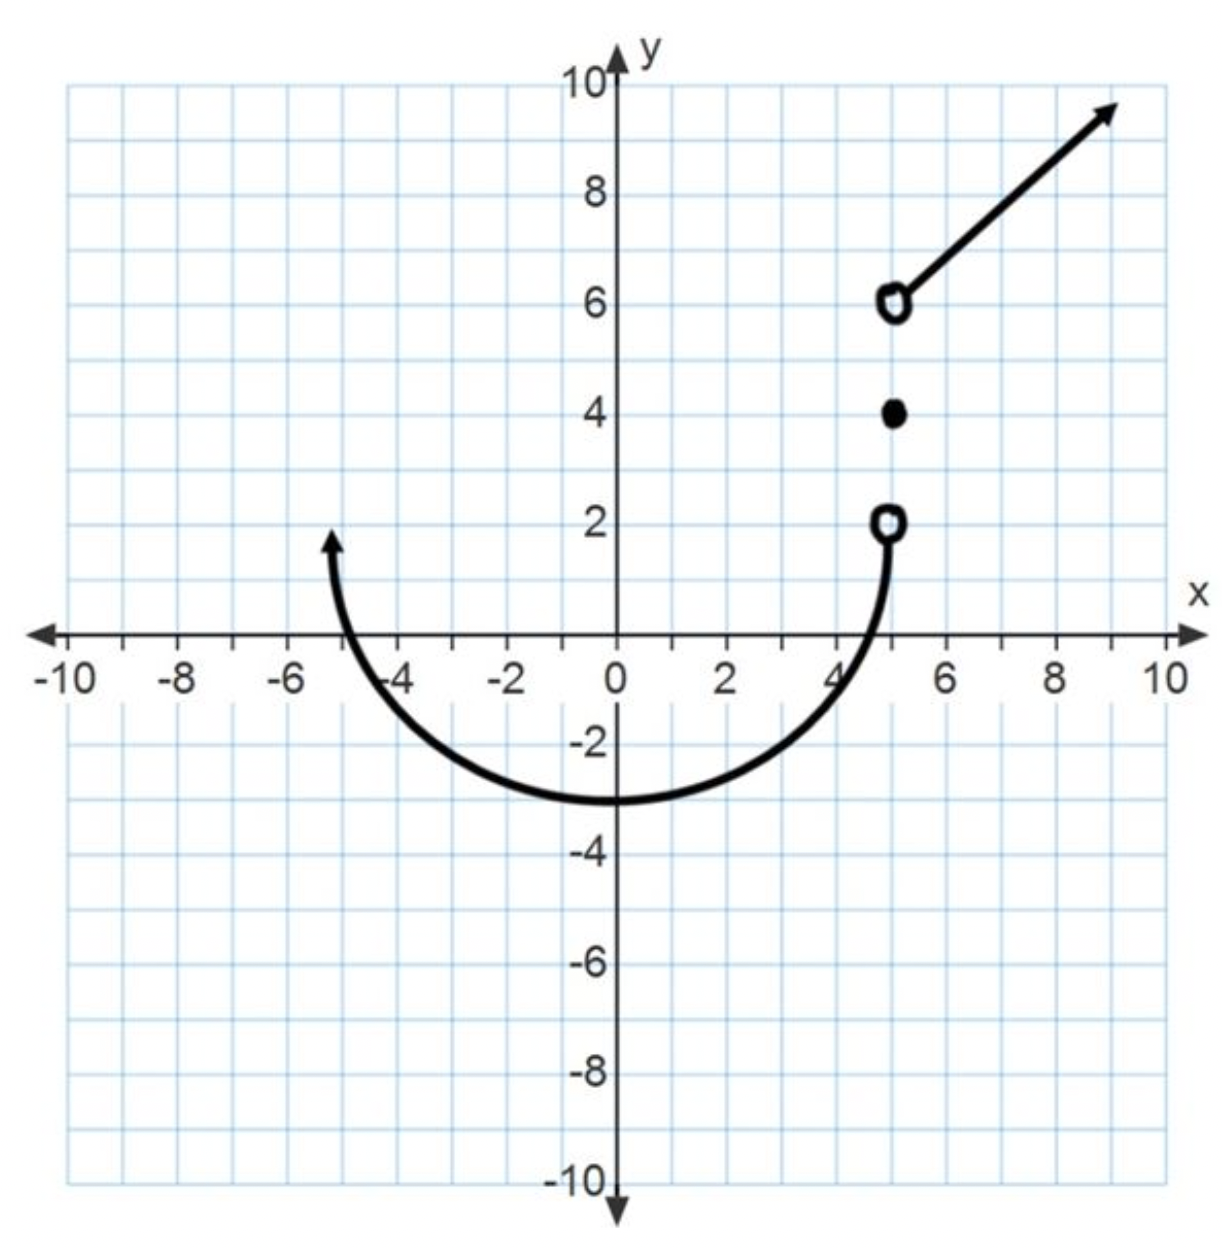
\includegraphics[width=0.5\textwidth]{graph2.png}

\begin{itemize}
    \item $f(5)$
    \begin{expandable}
        Value: $4$
    \end{expandable}
    \item $\lim_{x\to5^+} f(x)$
    \begin{foldable}
        Value: $6$
    \end{foldable}
    \item $\lim_{x\to5^-} f(x)$
    \begin{expandable}
        Value: $2$
    \end{expandable}
\end{itemize}

\end{document}